\def\year{2015}
%File: formatting-instruction.tex
\documentclass[letterpaper]{article}
\usepackage{aaai}
\usepackage{times}
\usepackage{helvet}
\usepackage{courier}
\usepackage{graphicx}
\usepackage{cleveref}
\frenchspacing
\setlength{\pdfpagewidth}{8.5in}
\setlength{\pdfpageheight}{11in}
\pdfinfo{
/Title (Human-Robot Collaboration: Affect-Driven Functional Coexistence)
/Author (Mahni Shayganfar, Charles Rich, Candace Sidner)}
\setcounter{secnumdepth}{0}  
 \begin{document}
% The file aaai.sty is the style file for AAAI Press 
% proceedings, working notes, and technical reports.
%
\title{Human-Robot Collaboration: Affect-Driven Functional Coexistence}
\author{Mahni Shayganfar, Charles Rich, Candace Sidner\\
Worcester Polytechnic Institute\\
Fuller Laboratories, 100 Institute Road\\
Worcester, Massachusetts, 01609\\
}
\maketitle
\begin{abstract}
\begin{quote}
We investigate the mutual influence of affective and collaboration processes in
a cognitive theory to support the interaction between humans and robots or
virtual agents. We will develop new algorithms for these processes, as well as a
new overall computational model for implementing collaborative robots and
agents. We build primarily on the \textit{cognitive appraisal} theory of
emotions \cite{gratch:domain-independent} and the \textit{SharedPlans} theory
\cite{grosz:plans-discourse} of collaboration to investigate the structure,
fundamental processes and functions of emotions in a collaboration context. As
part of this work, we also address a deficiency in existing cognitive models by
accounting for the influence of motivation on collaborative behaviors, such as
overcoming an impasse. This motivation mechanism uses the results of cognitive
appraisal to dynamically form new intentions related to the collaboration
structure.
\end{quote}
\end{abstract}

Intelligence is a set of mental abilities that enables a human to comprehend,
reason and adapt in the environment, and as a result, act effectively and
purposefully in that environment. Emotions play a crucial role in humans'
explanation of intelligent behaviors. Emotions affect not only what people do,
but also the way they do it \cite{cowie:concepts-definitions}. Ronald De Sousa
in The Rationality of Emotion \cite{sousa:rationality-emotion} makes a good case
for the claim that humans are capable of rationality largely because they are
creatures with emotions. Emotions significantly impact the procedures of action
generation, execution, control, and interpretation \cite{zhu:emotion-action} in
different environments. 

Emotions are conceptualized as ongoing processes rooted in dynamic social
contexts, which can shape both implicit and explicit emotional responses
\cite{parkinson:emotion-social-interaction}. Emotions are dynamic episode that
not only makes changes in cognitive states, but also produces a sequence of
response patterns on body movements, posture, voice and face
\cite{scherer:expression-appraisal}. Emotions typically occur in response to an
event, usually a social event, real, remembered, anticipated, or imagined. They
are associated with distinctive relational meanings
\cite{parkinson:holds-emotion}. These relations can be with the individual's
past experience, the individual's surrounding objects and environment, or the
other individuals with or without mutual beliefs in a dyadic or a group setting.
Emotions are evaluative and responsive patterns that serve the function of
providing appraisal about whether the ongoing event is harmful, threatening or
beneficial for the well-being of an individual \cite{zhu:emotion-action}.
Consequently, reasoning and emotional processes have an integral and a
supportive relationship, rather than an antagonistic and a conflicting one.

The idea of having robots or other intelligent agents living in a human
environment has been a persistent dream from science fiction books to artificial
intelligence and robotics laboratories. However, there are many challenges in
achieving collaboration between robots and humans in the same environment. Some
of these challenges involve physical requirements, some involve cognitive
requirements, and some involve social requirements. Thus far, there has been an
emphasis on the design of robots to deal with the physical requirements. Many
researchers are also working on the cognitive requirements, inspired by a
diverse set of disciplines. As time passes, there is an increasing recognition
of the importance of the social requirements, and how cognitive systems can
include the influence of the others.

\section{Motivation}

Functionnal coexistence is an important aspect of the symbiotic cognitive
systems in social environments. Collaboration requires coexistence with
the others and it also describes how a cognitive agent can function in such
environment. Therefore, the ability of collaborating with humans in the same
environment is crucial for cognitive agents. In fact, a cognitive agent's
ability to understand the collaborative environment impact the effectiveness of a
collaboration. Examples of cognitive capabilities that support the effectiveness
of collaboration include: a) perceiving one's own internal states and b)
communicating them, c) coordinating personal and group behaviors, d) identifying
self and mutual interests, e) recognizing the accountability of private and
shared goals, f) selecting appropriate actions with respect to events, and g)
engaging others in collaboration.

We are investigating the cognitive processes involved in a collaboration in the
context of a cognitive architecture. There are several well-developed cognitive
architectures, e.g., Soar \cite{laird:soar} and ACT-R \cite{anderson:act-r},
each with different approaches to defining the basic cognitive and perceptual
operations. There have also been efforts to integrate affect into these
architectures \cite{dancy:actR-physiology-affect,marinier:behavior-emotion}. In
general, however, these cognitive architectures do not focus on processes to
specifically produce emotion-regulated goal-driven collaborative behaviors. At
the same time, existing collaboration theories, e.g., SharedPlans theory
\cite{grosz:plans-discourse}, focus on describing the structure of a
collaboration in terms of fundamental mental states, e.g., mutual beliefs or
intentions. However, they do not describe the associated processes, their
relationships, and their influences on each other. In contrast,
\textit{Affective Motivational Collaboration Theory} deals with the major
processes, including affective and motivational processes, having an impact on
the collaboration structure. This theory is informed by research in psychology
and artificial intelligence. Our contribution, generally speaking, will be to
synthesize prior work on motivation, appraisal and collaboration, and thus to
provide a new theory which describes the prominent emotion-regulated goal-driven
phenomena in a dyadic collaboration.

\section{Social Functions of Emotions}

\section{Affect and Collaboration}

Collaboration is a coordinated activity in which the participants work jointly
to satisfy a shared goal \cite{grosz:plans-discourse}. There are many important
unanswered questions about the involvement of an individual's cognitive
abilities during collaboration. Some of these questions are related to the
dynamics of collaboration, as well as the underlying mechanisms and processes.
For instance, a general mechanism has yet to be developed that allows an agent
to initiate proactive collaborative behaviors when it faces a blocked task.
There is also a lack of a general mechanism that, in the event of a task
failure, allows an agent to consider the collaborator's anticipated mental
states and emotions, while managing its own internal goals and the
collaboration's shared goal. There are also other questions about the components
involved in these processes at the cognitive level, such as the processes that
are involved for evaluative, regulatory or motivative purposes. There has also
not been enough attention on the processes that are involved to maintain the
social aspects of a collaboration.

Emotions have a key role in influencing the cognitive processes involved in
social interaction and collaboration. Emotion processing and decision-making are
integral aspects of daily life and maintain their prominence during social
interaction and collaboration. However, researchers' understanding of the
interaction between emotions and collaborative behaviors is limited. We believe
that the evaluative role of emotions, as a part of cognitive processes, helps an
agent to perform appropriate behaviors during a collaboration. To work jointly
in a coordinated activity, participants (collaborators) act based on their own
understanding of the world and the anticipated mental states of the counterpart;
this understanding is reflected in their collaborative behaviors. Emotions are
pivotal in the collaboration context, since their regulatory and motivational
roles enhance an individual's autonomy and adaptation as well as his/her
coordination and communication competencies in a dynamic, uncertain and
resource-limited environment.

\section{Affective Motivational Collaboration Theory}

We are building Affective Motivational Collaboration Theory on the foundations
of the \textit{SharedPlans} theory of collaboration \cite{grosz:plans-discourse}
and the \textit{cognitive appraisal} theory of emotions
\cite{gratch:domain-independent}. Affective Motivational Collaboration Theory is
about the interpretation and prediction of observable behaviors in a dyadic
collaborative interaction. The theory focuses on the processes regulated by
emotional states. The observable behaviors represent the outcome of reactive and
deliberative processes related to the interpretation of the self's relationship
to the collaborative environment. Affective Motivational Collaboration Theory
aims to explain both rapid emotional reactions to events as well as slower, more
deliberative responses. The reactive and deliberative processes are triggered by
two types of events: \textit{external} events, such as the other's
\textit{utterances} and \textit{primitive actions}, and \textit{internal}
events, comprising changes in the self's mental states, such as belief formation
and emotional changes. Affective Motivational Collaboration Theory explains how
emotions regulate the underlying processes when these events occur during
collaboration. This theory elucidates the role of motives as goal-driven
emotion-regulated constructs with which an agent can form new intentions to cope
with internal and external events.

Affective Motivational Collaboration Theory explains the functions of emotions
in a dyadic collaboration and show how affective mechanisms can coordinate
social interactions by enabling one to anticipate other's emotions, beliefs and
intentions. Our focus is on the mechanisms depicted as mental processes in
Figure \ref{fig:cpm} along with the mental states. The \textit{Mental States}
includes self's (robot's) beliefs, intentions, motives, goals and emotion
instances as well as the anticipated Mental States of the other (human). The
\textit{Collaboration} mechanism maintains constraints on actions, including
task states and the ordering of tasks. The \textit{Collaboration} mechanism also
provides processes to update and monitor the shared plan. The \textit{Appraisal}
mechanism is responsible for evaluating changes in the self's Mental States, the
anticipated Mental States of the other, and the state of the collaboration
environment. The \textit{Coping} mechanism provides the self with different
coping strategies associated with changes in the self's mental states with
respect to the state of the collaboration. The \textit{Motivation} mechanism
operates whenever the self a) requires a new motive to overcome an internal
impasse in an ongoing task, or b) wants to provide an external motive to the
other when the other faces a problem in a task. The \textit{Theory of Mind}
mechanism is the mechanism that infers a model of the other's anticipated mental
state. The self progressively updates this model during the collaboration.

\begin{figure}[tbh]
  \centering
  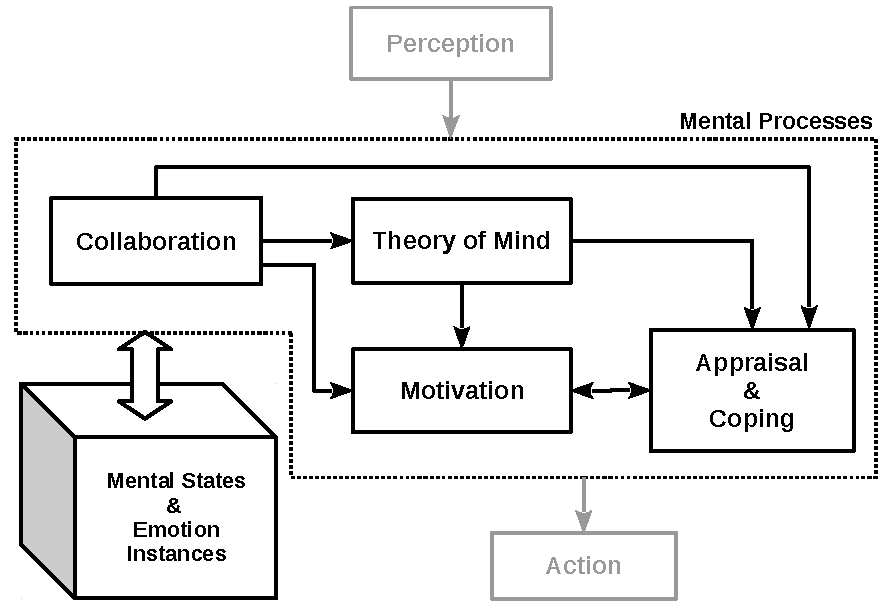
\includegraphics[width=0.474\textwidth]{figure/theory-general-croped.pdf}
  \caption{Computational framework based on Affective Motivational Collaboration
  Theory (arrows indicate primary influences between mechanisms).}
  \label{fig:cpm}
\end{figure}

\section{Functions of Emotions}

Emotions have a crucial role in communicating one's mental state, motivating
one's actions, and evaluating and interpreting their internal states and the
environment. Emotions generally speaking provide a set of intra- and
interpersonal functions which regulate internal processes and the self's
relationship to the other during the collaboration. An emotion instance, e.g.,
\textit{anger}, occurring during collaboration, can lead to different emotion
functions, e.g., \textit{Alarm Mechanism} and \textit{Action Selection}.
Emotions have meanings in a social context which can be interpreted by an
observer. Emotion functions are important because they provide social
characteristics that the self needs to manifest in its collaborative behavior. 

\section{Collaborative Behaviors in Symbiotic Environments}

Collaboration is a coordinated social activity in which participants work
together to perform tasks achieving a shared goal. Collaborative behaviors
enable individuals to work together in a shared environment. These behaviors
help an observor to distinguish between collaboration and other social or
group activities. For instance, collaborators need to be able to synchronize
themselves with their partner and collaborative environment with respect to the
state of the shared goal. To generate collaborative behaviors one requires to
include certain computational mechanisms. Affective Motivational Collaboration
Theory provides affect-regulated goal-driven mechanisms (see Figure
\ref{fig:cpm}) by which a robot will be able to show collaborative behaviors. In
the followings, we breifly describe eight different social characteristics of
collaboration and how they are related to emotion functions.

\begin{itemize}
  \item \textbf{Awareness}
  \item \textbf{Motivation}
  \item \textbf{Self-synchronization}
  \item \textbf{Participation}
  \item \textbf{Mediation}
  \item \textbf{Reciprocity}
  \item \textbf{Reflection}
  \item \textbf{Engagement}
\end{itemize}

\subsection{Awareness} Awareness is the self's ability to manage and understand
its own emotions and those of the other, and the ability to express emotions
accordingly. Managing emotions refers to the self's capacity to regulate its
internal emotions and to direct them towards constructive activities. Emotions,
as a crucial evaluative substance of the cognition, can increase the
accessibility and significance of discrepancies between Mental States, leading
to higher awareness of one's sense of self and one's collaborator. In my theory,
beliefs about the outcome of the appraisal and reverse appraisal
\cite{gratch:reverse-appraisal} provide an internal and social understanding of
the world. Ultimately, the self and social awareness helps our agent to become
part of a collaboration process, while adopting and maintaining a shared goal.

\subsection{Motivation} Motivation as a social characteristics of collaboration
is goal-driven and concerned with self's actions and what determines those
actions. There are several motivation theories describing various functional
aspects of motivations. These theories can be categorized into two different
groups, the \textit{self-regulatory} and the \textit{purposive} motivations
\cite{graham:motivation}. As a regulatory process, motivation restores internal
cognitive equilibrium of the self as well as self's social stance during
collaboration. From a purposive perspective, the motivation process emphasizes
the goal-directed nature of behaviors by anticipating the utility of self's
individual actions or series of actions reaching to the private or the shared
goal. In both self-regulatory and purposive perspectives, emotions serve the
Motivation mechanism, offering their evaluative nature to assess the internal
and external events. This process drives our agent to gain consensus in problem
solving or development during collaboration.

\subsection{Self-synchronization} Self-synchronization represents the temporal
and spatial relationship of the self with the collaboration environment
\cite{manso:synchronization}. Adaptation as a function of emotions (see Section
\ref{emotion-functions}) play a crucial role in short and long-term behavior
changes in our agent enabling self-synchronization. Furthermore, the sensory
integration function of emotions can impact the synchronization procedure in
the sensory level by filtering or blocking of the input data. For instance, the
self can perceive the other's anger and consequently infers that the other will
not totally pay attention to what the self says. The prominent role of emotions
in the synchronization process during collaboration extends to their other
functions in different levels of cognition including action selection, not only
based on a plan but according to the self's emotional states; goal management,
whenever a new goal or a sub-goal is required to be created or reprioritized;
alarm mechanisms for informing the self by interrupting other cognitive
processes; attentional focus, by changing the self's focus of attention between
different existing saliencies in the collaboration environment; and strategic
processing, by influencing the actual decision making processes of the self. As
a result, our agent decides when things need to happen during the course of a
collaboration.

\subsection{Participation} It is suggested that the benefits of the
collaboration arise from active participation in interaction and verbal
communication with a partner who has a different perspective, either due to more
knowledge, or a different viewpoint \cite{kruger:peer-collaboration}. Active
participation in doing tasks and communicating during the collaboration is
directly related to the evaluative factors of one's cognitive processes. These
evaluative factors are intertwined with different aspects of performance
assessment hinged on the core concept of the collaboration, the shared goal . In
order to achieve the shared goal, the self employs the evaluative nature of the
appraisal process to be able to assess and participate in the ongoing
collaboration. Emotion instances provide appropriate, accountable and
communicative signals (verbal and non-verbal behaviors) both for the self,
through the manipulation of the Appraisal and Belief Formation mechanisms, and
for the other, through the multi-modal emotional expressions which make the
other socially aware of the self's internal states. Consequently, our agent
participates in collaboration while expecting the other to participate to
achieve the shared goal together.

\subsection{Mediation} Collaborations can include disputes needed to be
intervened and solved by the collaborators. Negotiation is the bargaining
process between parties seeking to discover a common ground and reach an
agreement to settle a matter of mutual concern or resolve a conflict.
Collaborative negotiation is an interest-based, constructive negotiation (as
oppose to competitive negotiation) in which the self and the other are
seeking a fair and equitable agreement without having an always-conceding
approach. During the collaborative negotiation the collaboration parties openly
discuss their needs and try to create as much mutual value as they can.
Therefore, the collaborators try to use and understand the feelings, deeper
interests and motives of their collaboration partner as well as their own.
Emotions, once again, become important for the self in assessing the
other's offers and counter offers. Additionally, the self can
communicate the result of this internal assessment through the expression of
emotion instances. In the inverse of the same procedure, the reverse appraisal
assists the self to perceive and interpret the other's emotional
expressions and observable behaviors. Hence, our agent would be able to assess
the negotiation events and to communicate its internal states during negotiation
and therefore, find a middle ground according to the mutual interests and
agreements.

\subsection{Reciprocity} Reciprocity is an adaptation process by which
individuals monitor their contributions in light of their partner's
contributions and make adjustments accordingly
\cite{cole:reciprocity-collaboration}. Reciprocity is fundamental for creating
mutually beneficial and non-zero-sum outcomes through social exchange of
resources and coordination of joint activities. In fact, the adaptations
associated with coordination using mutual beliefs and the shared goal concepts
create a different, yet another important aspect of the reciprocity in
collaboration. It leads to punishment or avoidance of collaborators with
detrimental actions and to reward in contrasting situations.
  
There are several underlying mechanisms helping the self to perform reciprocal
behaviors \cite{cole:reciprocity-collaboration}. First, a tacit \textit{resource
monitoring mechanism} is required for the self to monitor its own as well as the
other's resources contributions over the course of the collaboration. This
monitoring process essentially requires the existence of an assessment process
on collaborators' behaviors. The Appraisal mechanism provides this required
evaluative functionality. This notion of evaluation process helps the self to a)
perceive other's affective responses, and b) communicate its own. Second, a
\textit{reciprocal behavior failure detection mechanism} is needed to detect the
other's failure in vital reciprocal situations (which can be met with the
guidance of the Appraisal mechanism). Third, a \textit{resource adjustment
mechanism} is crucial for a collaborative agent to adjust its own social
exchange behavior and also to influence the other's reciprocal behavior. The
self can apply the emotion instances, e.g., guilt and gratitude, as
inducements to get the other to return favors. The same mechanism, e.g., anger
and sadness, can be applied by the self to punish or avoid the other based on
his behavior. As a result, our agent will share resources and thoughts, and will
expect sharing in return through reciprocity.

\subsection{Reflection} Reflection is an attempt to make the implicit, explicit
in order to learn from experience. There are two different types of reflection
\cite{schon:reflection}. The first, \textit{reflecting on action}, helps the
self to think back on behaviors of the other occurring because of the
self's last action. This process uses the Appraisal mechanism to evaluate the
other's response, and serves the self by reshaping what the self does,
by modification of the underlying beliefs and intentions. Additionally,
reflection helps the self to learn the consequences of each action, using the
content of its own Mental States, including beliefs about the other's
Mental States. Consequently, the outcome of this evaluation enables the self
to update its user model of the other. These processes represent the
deliberative side of the emotion functions. The second type of reflection,
\textit{reflecting in action}, helps the self when a familiar routine produces
an unexpected result; an error stubbornly resists correction; or, the meaning of
an event has changed because of changes in the self's evaluative and/or
interpretive processes. All these changes produce pleasant or unpleasant results
for the self leading to different emotion instances, e.g., surprise, during
collaboration. The self can intentionally ignore the events signaling these
emotions and not attempt to change its own focus of attention, or in contrast,
can show a quick emotional reaction, for instance because of the occurrence of
an unexpected event, in which the latter represents the reflexive function of
emotions. Subsequently our agent can process the collaboration status and
consider alternative actions at each point in time, when required.

\subsection{Engagement} There are three different forms of engagement:
\textit{behavioral, emotional} and \textit{cognitive} engagements
\cite{appleton:engagement}. The \textit{behavioral engagement} is associated
with self's sustained behavioral involvement by taking actions during
collaboration. The self's behaviors that can be indicative of behavioral
engagement include persistence in taking actions, maintaining the focus of
attention during collaboration, asking questions from the other whenever
it is required in the current state of the world, and contributing to achieving
the shared goal. The \textit{emotional engagement} is associated with self's
emotional reactions to its collaborator. These reactions are aimed at showing
empathy to the other in different cases, for instance, the occurrence of
the failure or disruption in one of the collaborators' tasks, e.g., anger or
frustration. In general, the self can empathize with the other in the
event of the appearance of any anticipated negative emotion. The emotional
engagement can also help the self to evaluate the level of satisfaction based
on the performance of the individual tasks from its own and the other's
point of view. This evaluative process will help the Motivation mechanism to
form the most appropriate intention to maximize the performance of the
collaboration according to the shared plan. The \textit{cognitive engagement} is
associated with whether the self is willing to get involved in solving problems
occurred during the collaboration. The Appraisal and the Motivation mechanisms
serve the self to evaluate the status of the collaboration and form new
intentions for actions. The Intention Formation process helps the self to find
the proper solution for an ongoing issue even if the action is a part of the
other's task. Consequently, our agent will proactively engage in cases
when an unexpected problem occurs during collaboration, rather than just waiting
to see what the other's demand is.

\section{Conclusion}

\bibliography{mshayganfar.bib}
\bibliographystyle{aaai}

\end{document}
